% !TEX encoding = UTF-8 Unicode
% !TEX program = pdflatex
% !TEX spellcheck = en_US


% In order to correctly compile this document,
% execute the following commands:
% 1. pdflatex
% 2. pdflatex
% 3. pdflatex



\documentclass[amsthm,ebook]{saparticle}

% IF YOU USE PDFLATEX
\usepackage[utf8x]{inputenc}
% if you write in english and in greek
\usepackage{ucs}
\usepackage[greek,english]{babel}
\languageattribute{greek}{polutoniko}

% IF YOU USE XELATEX
%\usepackage{polyglossia}
% if you write in italian
%\setmainlanguage{italian}
% If you want put some ancient greek:
%\setotherlanguage[variant=polytonic]{greek}
%\newfontfamily{\greekfont}[Ligatures=TeX]{Palatino Linotype}

% dummy text (remove in a normal thesis)
% remove if not necessary
\usepackage{siunitx}
%Natbib for bibliography management
\usepackage[authoryear]{natbib}
% custom commands
\newcommand{\bs}{\textbackslash}

%%%%%%%%
%TITLE:%
%%%%%%%%
\title{Mapping Epigraphic Databases to EpiDoc}

%%%%%%%%
%AUTHORS:%
%%%%%%%%
\author[UHEI]{Liuzzo Pietro\corref{first}}

\cortext[first]{Corresponding author. Email: pietro.liuzzo@zaw.uni-heidelberg.de}

\address[UHEI]{Ruprecht-Karls-Universität Heidelberg - Marstallstraße 6, 69117, Heidelberg (DE)}

\begin{document}
\maketitle

\begin{abstract}
The Europeana network of Ancient Greek and Latin Epigraphy brings
together most repositories of ancient epigraphic material and aims to
provide historians not just with a useful research tool, but a
curated online edition which has high quality content as well as high
quality data.  In this paper some of the up-conversion, alignment and enrichment tasks are presented.
 
\end{abstract}

\keywords{EpiDoc, XML, Vocabularies, Linked Data, Data harmonization}

\section{Introduction}\label{sec:intro}


The Europeana network of Ancient Greek and Latin Epigraphy\footnote{\citet{OrlandiCasarosa2014} \citet{Orlandi2014} \citet{liuzzo2014} \url{http://www.eagle-network.eu/}} brings
together most repositories of ancient epigraphic material and aims to
provide historians not just with a useful research tool, but a
curated online edition which has high quality contents as well as high
quality data. Towards this end many steps are needed as the databases on which many institutions have worked for decades cannot be just discarded. Epigraphy enjoys a special position among digital resources as most transcriptions of existing classical inscriptions have been digitized. Many duplicates exist and a lot of the content lacks metadata almost entirely, but the work continues with dedication so that among the 10 \% of digitised European Cultural Heritage, Ancient Epigraphy can certainly claim to play a strong role.\footnote{The data is taken from the Europeana 2020 strategy report available at \url{http://strategy2020.europeana.eu/}.} While the long term aim for epigraphy is on the one hand to keep up with new finds and studies and on the other to have a common and flexible entry point and backend on which to work together, this is not easy to accomplish without a careful process which involves a gradual transition from independent databases (the best option at the time when the EAGLE databases were created) to a common online data entry and editing system working on XML files in EpiDoc, as it has now become feasible.   
In this paper some of the mapping and content harmonization efforts undertaken by the EAGLE BPN to achieve this step towards a common epigraphic resource, will be presented as a case in which this apparently technical task involved deep revision of contents related to the discipline and required discussions and collaborative efforts by the working
groups of digital epigraphists, encoders, epigraphists and developers, coming from several different background and experiences. The result of this work are the automated conversion to TEI EpiDoc XML of 90\% of the text features in the EAGLE databases and the EAGLE Vocabularies, the largest existing controlled and aligned vocabularies for classical epigraphy.\footnote{\url{http://www.eagle-network.eu/resources/vocabularies/}} 

\section{Why XML}
Choosing XML for an online publication is almost obvious given the current stage of development of the editorial methodology in epigraphy. However there is room for a brief explanation of why this is preferable on a large scale to a relational database. I would like to suggest a comparison here. Coffee is produced by filtering water through a powder more or less thick. This can be accomplished by pushing water through the coffee (as in most systems, from a mocha to an espresso machine) or coffee through the water (as in a french press, where the coffee floats and is pushed down). There is pretty much the same difference when we compare the action of entering data into a database, i.e. a rigid structure of information, and marking up a text, adding tags to the text itself. The first process forces data through a grid however well thought off, while in the second case structure is added on the contents without altering them, but just enhancing their potential so that the richness and values of both contents and structure empower each other. There is just more taste and much more freedom of encoding to the level desired and to the complexity one wants. An additional advantage is the level of interoperability. An XML file is virtually software independent, it is not an Access, FileMaker or whatever database format. A third reason is that an XML file can host a complete textual description with semantic markup and still have the structure of a normal text edition, while the same source can be used to produce a database or an index for interrogation purposes. For example the same markup of an abbreviation \texttt{<expan><abbr>C</abbr><ex>aio</ex></expan>} can be used to produce a database of abbreviation marks and expansions, to output in a diplomatic edition only the character actually on the stone or to print the expanded abbreviation in a critical edition.\footnote{\url{http://www.stoa.org/epidoc/gl/latest/trans-abbrevmark.html}} To print a database to a book would be at least more cumbersome. XML provides also a better service as an archival format being explicit on the values it uses to describe contents, moreover if these follow a schema of agreed value of such elements. This said producing and sharing XML files means that more quality editions can be produced, printed editions can be produced and all sort of outputs can be supported with flexibility; it means that data is safe from software developments and support; it means you don't have to put information into a rigid table which is then hard to restructure, but that you can annotate your text as much as you want thus adding layers and layers of ``possible databases'' of relevant information to be extracted and used.   
The text is what one uses to describe situations and complexities, the markup allows also the machine to know and retrieve that information as in a database: you don't need a field or an element to state what the orientation of your text is, you can simply state and describe as you would do in a normal publication and if you want to reuse information about the text orientation then you can add elements and attributes to do so. XML allows not to worry too much on ``what goes where'' or about ``where do I put that info" because it is not a database, so that the editor can instead focus on ``what is that'' and on accurately describing it. The TEI specification which is EpiDoc allows the specific epigraphic content to be described fully for what concerns the text of inscriptions, drawing on more than a decade long experimenting and development of this standard thanks to a vast and active international community. The simple fact of using the same markup to describe our texts allows us to study them together and to produce and run software for more then just one corpus of inscriptions. 

\section{EAGLE Mappings and Metadata modeling}
The EAGLE BPN has taken 18 different content providers and has come to
the decision to take the first steps to bring hundreds of thousands of
ancient Greek and Roman inscriptions to TEI. This required 14 mappings
of local database metadata models to TEI/EpiDoc, as well as the elaboration of
XSL Transformations\footnote{\url{https://github.com/EAGLE-BPN}} for up-conversion\footnote{This is the terminology used by \citet[906]{Kay} to describe transforming without explicit structure in data which has it. In this case it is a transformation from a less explicit database structure to a fully explicit and interoperable one.} and the alignment of the text
markup. Although this was thought to be a trivial task it turned out
that whereas databases claimed to use the same conventions, a considerable amount of differentiation took place due to the data structure and to data entry procedures as well as to policies and internal decisions. 

The main harmonization task undertaken has been to align the XML format
of data provided for aggregation and ingestion, to the TEI
specification EpiDoc.\footnote{\url{http://www.stoa.org/epidoc/gl/latest/}} This well established TEI schema, broadly used in
many high quality projects, allows for a very easy alignment, for the
production of an XML file compliant with international standards and
for high flexibility for integration of the vocabularies and places
gazetteer in use.

Moving from a database to a marked up text is a partially mechanical operation which involves a theoretical jump. As coffee is better when water goes through coffee powder rather than when coffee goes through the water (as in a french press), a database has fields to be filled, while marking up a text is a descriptive activity which is attached to information whichever textual form it takes.\footnote{See above.} Mapping from a database to XML forces into the XML a structure and a logic which is that of a database, whereas the freedom and flexibility achieved with XML are yet to be actually realized and exploited.  

In order to offer a complete and critically structured endpoint to the user on the side of data, to describe inscriptions and their representations, EAGLE considered beside TEI also CIDOC CRM, studying and providing a full EpiDoc to CIDOC-CRM mapping.\footnote{Still under development, within the ARIADNE project. \url{http://www.ariadne-infrastructure.eu/}. The need for a working group and a variant declension of CIDOC for epigraphy have been highlighted during the Nicosia EAGLE meeting in March 2015.} This would have enabled a further full description in a different logic, that of the web of data, but the attempts made proved the need for more specific efforts.

There are several mappings involved in the aggregation work of EAGLE. Content providers need to map to a common Eagle Metadata Format, and the data produced will then be mapped to the Europeana Data Model\footnote{\citet{D3.1}} in order to be aggregated in Europeana, for a wider dissemination with a special eye for the general user.


\section{EAGLE Metadata Model and Harmonization}

The occasion of a mapping work allows also for other tasks of curation to be performed.
EAGLE Members had in some case the text of a same inscription with three parallel different types of encoding conventions applied.

\begin{figure}[htbp] 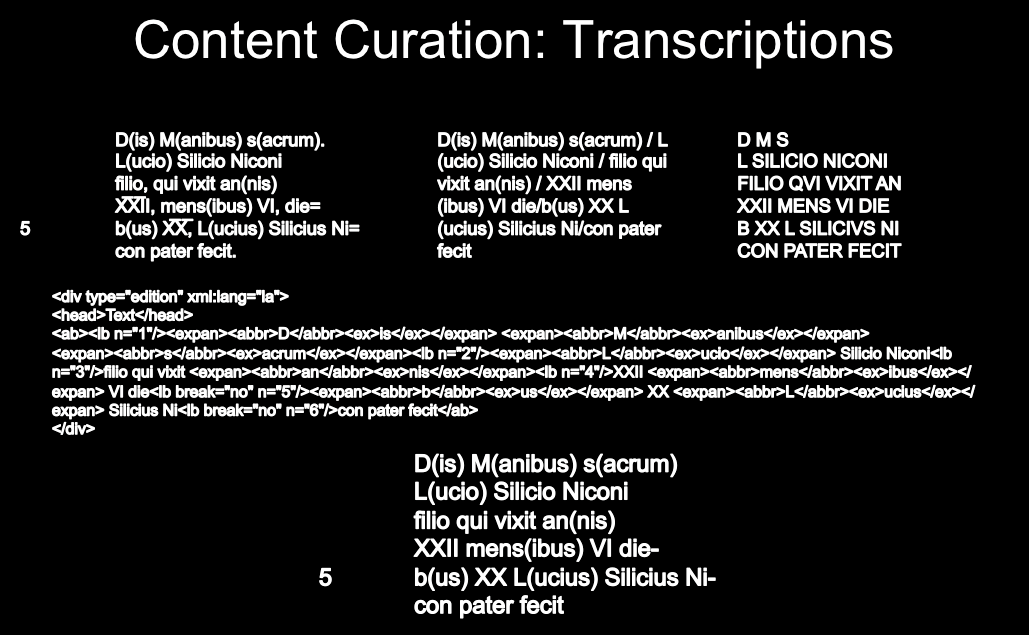
\includegraphics[width=\columnwidth]{Contentcuration.png} \caption[]{Different Texts before and after harmonization though up-conversion} \end{figure}

In the context of the mapping to EpiDoc of the metadata, the text also underwent transformation with tools which have been developed to support the alignment and harmonization of data from content providers to international standards for what concerns digital editions of inscriptions.

Given the template described in Part III, and ANNEX II of the EAGLE Metadata Schema (\citet{D3.1}), an XSL Transformation converts from string epigraphic texts in marked up TEI-EPIDOC XML, following the \href{http://www.stoa.org/epidoc/gl/dev/}{EpiDoc guidelines} (\citet{Elliott2007}).

These XSLT:\footnote{Based on Chetc.txt (by Hugh Cayless, Elli Mylonas, Gabriel Bodard and Tom Elliott) and further support from the Epidoc Collaborative (especially from Gabriel Bodard)} 

\begin{enumerate}
\item allow the conversion of epigraphic texts with various encodings and conventions from string to Epidoc markup and valid against the The EpiDoc RelaxNG schema.
\item Populate appropriate elements with available common URI from the EAGLE vocabularies\footnote{\url{http://www.eagle-network.eu/resources/vocabularies/}}

\end{enumerate}

This export set up will also guarantee that contents are kept aligned to the EpiDoc guidelines at all stages guaranteeing an effort free alignment to these international conventions for partners who can continue to apply local conventions for editing. But I would like to give more details on the steps of this process as an example of how it was possible to extract semantics, entities, and patterns from these text while aligning metadata format to an internationally recognized standard.
\bigskip

\subsection{Step 1}
Each project uses different conventions and therefore the regular expressions used to match particular situations are different.
The process of mark up of the string text in div[@type="edition"] is accomplished in several steps to guarantee consistency and precision.

The \texttt{textstructure.xsl} looks for marker of different sections and tokenize them to apply the same XSLT to each section of the text which needs to be contained by an <ab> element. If there is only one part it applies following instructions to that only.

Each section of text is then processed by the \texttt{brackets.xsl}. Normalizing brackets is important for the following steps and splits individual semantic values. The notation [ort 3], which would mean that a supplied text is followed by a gap of three letters, is divided into [ort][3].

The normalized string which results from this process is then passed to the 
\texttt{up-conversion.xsl} which works using a specific operation to search for regular expressions patterns (\texttt{xsl:analyze-string}) and substitute them with correct xml elements.

Running the transformation on the pattern {\textless}E=F{\textgreater} will return the following result:

\begin{verbatim}

<choice><corr>E</corr><sic>F</sic></choice>

\end{verbatim}


The result of this template is then passed to a further template which gives consistent numbers (\texttt{insertnumbers.xsl}). Empty lines do not need to have numbers, so Xpath is used to evaluate where to put a 0 as value of the @n in the {\textless}lb{\textgreater} element. Starting from this

\begin{quotation}
{}-{}-{}-{}-{}-{}-] / e[t?] Q(-{}-{}-) Bl(a)e[sus?] / contub/ernalis / eius / d(e) s(uo) l(ibens) l(aetus) d(edit)
\end{quotation}

The result of this processes is then the following\footnote{The amount of feature supported is much higher and some example of complex text successfully converted can be seen in this presentation online}

\begin{verbatim}

<ab>
<lb n="0"/><gap reason="lost" extent="unknown" unit="line"/>
<lb n="1"/>e<supplied reason="lost" cert="low">t</supplied> 
<abbr>Q</abbr> 
Bl<expan><ex>a</ex><abbr>e</abbr></expan><supplied
reason="lost" cert="low">sus</supplied>
<lb n="2"/>contub
<lb break="no" n="3"/>ernalis
<lb n="4"/>eius
<lb n="5"/><expan><abbr>d</abbr><ex>e</ex></expan> 
<expan><abbr>s</abbr><ex>uo</ex></expan> 	
<expan><abbr>l</abbr><ex>ibens</ex></expan> 
<expan><abbr>l</abbr><ex>aetus</ex></expan> 	
<expan><abbr>d</abbr><ex>edit</ex></expan>
</ab>
\end{verbatim}


\subsection{Step 2}
On the elements which contain information such as Object Type, Material, Execution Technique, etc. which are typically handled with a controlled vocabulary a series of XSL transformations is passed, one for each vocabulary related to that element  to match the content of the element with the vocabulary entry into the SKOS vocabulary stored in git, regularly updated and published as a self standing resource on the EAGLE portal.\footnote{\url{http://www.eagle-network.eu/resources/vocabularies/}} What follows is a brief description of such vocabularies and their development.

\begin{figure}[htbp] 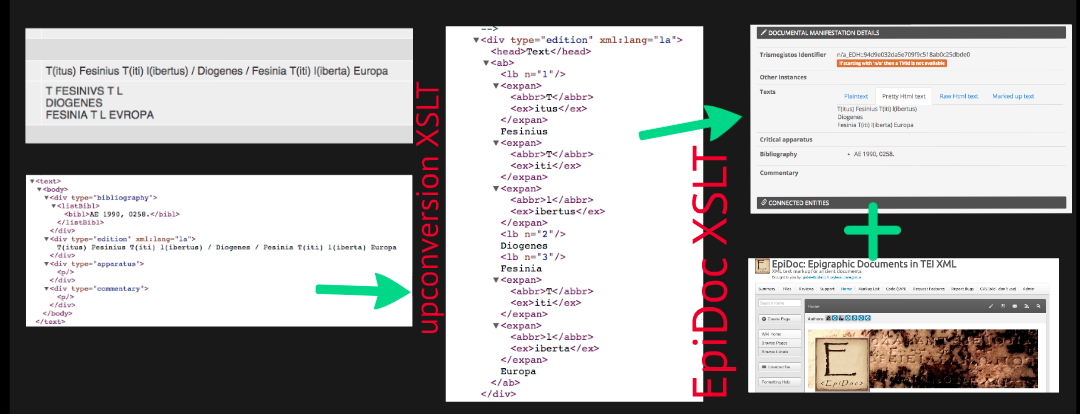
\includegraphics[width=\columnwidth]{upconversion.png} \caption[]{Stages of transformation of a text: database, template, up-conversion, checking and display with EpiDoc XSLT.} \end{figure}

\section{Classification problems: the EAGLE Vocabularies}
As Di Stefano Manzella \footnote{\citet[109]{Manzella1987}} clearly explained classification is no easy issue in any field: epigraphy is no exception to this rule. Traditionally the CIL VI (Rome) classification has been used as a reference, as this typology has served as a model for all epigraphic production in the Roman Empire. There are nevertheless new glossaries and classification curated by \href{http://cil.bbaw.de/cil_en/dateien/glossar.php#auswahlglossar}{CIL}, which retain the scientifically selective constraints of a formal classification, together with the benefits of this.

Problems are various, and include also the use of terms across vocabularies and the doubts which might be generated by archaeological chance.\footnote{ See \citet[XI-XII]{Piso}, following a current of studies which has its main in G. Susini and J.-N. Bonneville.}

What looks like an \href{http://www.eagle-network.eu/voc/objtyp/lod/29}{altar} could be also the \href{http://www.eagle-network.eu/voc/objtyp/lod/57}{base of a statue}, for example. Or perhaps it could have served two different function has an object of which we might or not have any archeological, contextual or textual trace.  

\begin{figure}[htbp] 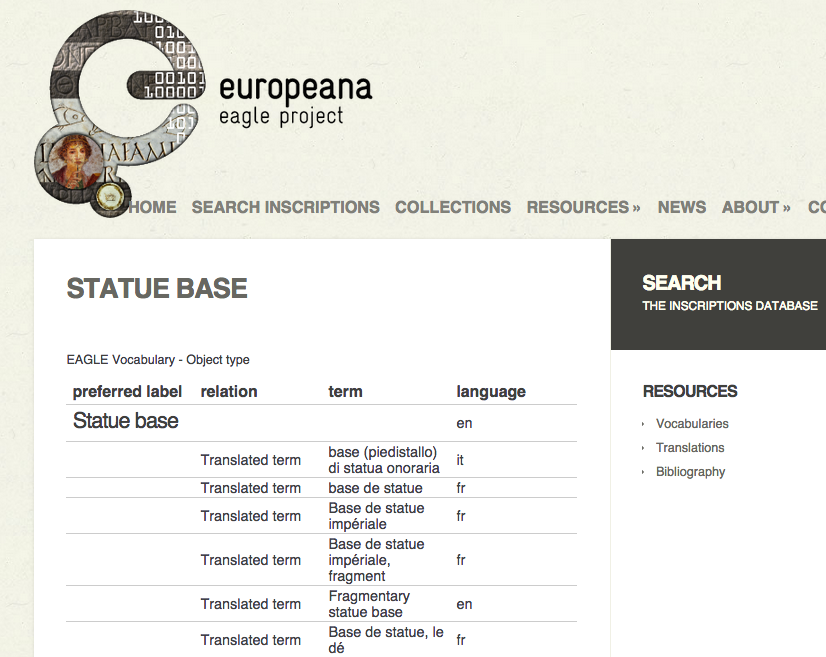
\includegraphics[width=\columnwidth]{statuebase.png} \caption[]{Statue Base} \end{figure}

This is also the case when we deal with techniques of execution of an inscription. Those can also be multiple and an inscription can be for example both a graffito and painted.
And this is just not to mention the extreme complications of having a lot of independent vocabularies, each one for its own sake and small scope purpose. This is often the best option for correct attribution as local habits do vary. But within the framework of harmonization activities, it is important to refer to connected and interrelated definition of terms (not univocal!) and to allow for multiple values to coexist. This is one best practice in the definition of vocabularies which is very important for the nature of content in question. 
This is also the reason why the EAGLE decided to provide not just definitions of all main terms but also examples from different areas and in different state of preservation, and as far as possible also bibliographic reference to authoritative sources.

The EAGLE Vocabularies are the following

\begin{itemize}
\item \href{http://www.eagle-network.eu/voc/typeins.html}{Type of Inscription}
\item \href{http://www.eagle-network.eu/voc/objtyp.html}{Object Type}
\item \href{http://www.eagle-network.eu/voc/material.html}{Material}
\item \href{http://www.eagle-network.eu/voc/writing.html}{Writing and Execution} 
\item \href{http://www.eagle-network.eu/voc/decor.html}{Decoration} 
\item \href{http://www.eagle-network.eu/voc/statepreserv.html}{State of Preservation} 
\item \href{http://www.eagle-network.eu/voc/dates.html}{Dating Criteria} 
\end{itemize}


\begin{figure}[htbp] 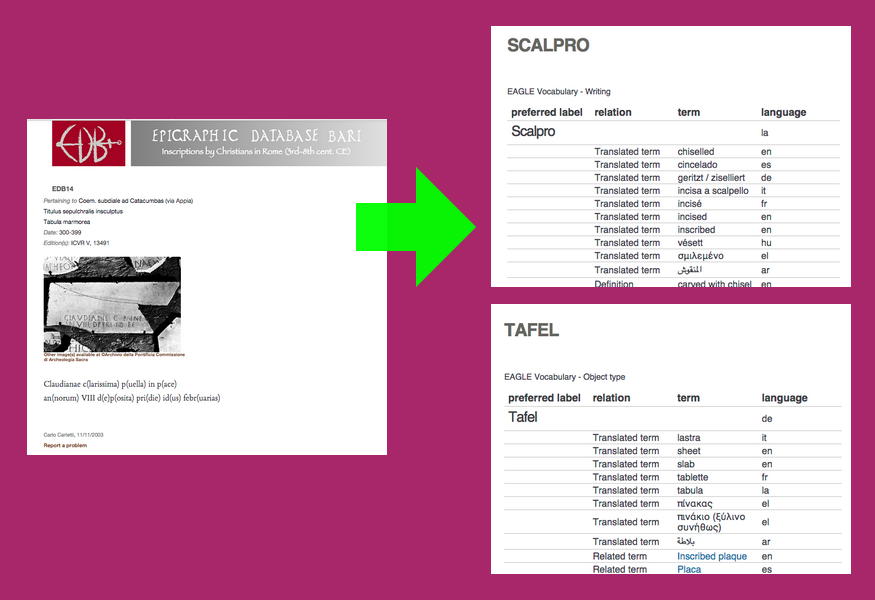
\includegraphics[width=\columnwidth]{edb.png} \caption[]{EAGLE Vocabularies used by the Epigraphic Database Bari} \end{figure}

The EAGLE vocabularies are maintained in a git repository where they are manually updated and transformed to a readable versions (with another XSLT transformation) published on the EAGLE website as a self standing resource linked to several others. A user is thus able to search for a type of object and read a definition as well as searching for more information on Wikipedia, Wikidata, Wikisource, etc. including the partners' websites. The Vocabularies perform thus both a technical function and are at the same time a living resource which can be read and used independently.

\section{Linked Open Data}
The Europeana LOD practice for metadata recommends the adoption of machine readable vocabularies. Within the EAGLE BPN Linked Open Data practices and approaches have been taken on board for a process which will bring current material some steps closer to that practice.\footnote{\citet{Bizer2009}} Addressing existing problems in classification and the publication of a machine readable vocabulary of values (controlled vocabulary) is one of these steps:\footnote{\citet[4-5]{Harper2012} for the definition. See also \citet{Isaac2012}} it involves identifying and matching values as well as giving them stable identifiers and making of them self standing resources where possible.

In facts the many problems and complexities which \citet{Manzella1987} underlined and exposed can find a solution using the LOD approach.\footnote{\citet{Bizer2009}} Both the limits of choices and hierarchical organization can be bypassed using unique identifiers and relations among those. Polyhierarchic structures as well as the presence of many possible denomination with specific and self standing definition allows for both precision, consistency and sustainability over time of this approach.\footnote{\citet{Harpring2010}} 

For example, an inscription can easily be classified both as \emph{magistrati populi romani} and as \emph{decuriones municipales}; a document can be classed both under the \emph{fasti} and under the individual mentioned in the text. These major advantages can be exploited when the effort of publishing open machine readable material is undertaken and a document can be then classified chronologically and alphabetically without the need of an authorial choice.\footnote{I would like to thank prof. Piso for input on this point, given during the work of the Working Group.}

Nevertheless, the major possible advantage is that there is no evident need, with a LOD approach, to distinguish among Greek and Latin inscriptions: they can find their place together in a Linked Data  edition and benefit of other efforts in this direction.


\section{Crosswalking EpiDoc to EDH with XSLT}
The proof of concept of usability of the XML source file is given by the reverse function being possible, i.e. to transform the XML files into a database data structure. A team of people from the EAGLE BPN\footnote{Gabriel Bodard, Pietro Liuzzo, James Cowey, Frank Grieshaber, Brigitte Gräf and Francisca Feraudi Gruénais.} and Scott Vanderbilt, curator of the online edition of the Roman Inscriptions of Britain,\footnote{\url{http://romaninscriptionsofbritain.org/}} worked on mapping the EpiDoc contents of that project to the EDH database model,\footnote{The work was largely based on the previous exercise of this kind, made by Gabriel Bodard and James Cowey for the Inscriptions of Roman Tripolitania.} facing a series of problems and challenges, which brought an interesting discussion, also on principles of ``up-conversion'' and cross-walking, which should be as often as possible multi-directional.\footnote{The files are available here: \url{https://raw.githubusercontent.com/EAGLE-BPN/Epidoc2EDH/master/rib_to_edh-2.xsl}}

Challenges included
\begin{itemize}
\item alignment to EDH internal vocabularies
\item alignment to EDH conventions for bibliographic references
\item use of internal references and retrieval of key based information
\item matching of existing items
\item formatting to EDH conventions differentiated based on the type of content extracted (text or names) 
\end{itemize}

The result was successful and proves once more if needed that an XML source format is a preferable option whatever the variety of desired output are.

\section{Conclusion}
I have presented in this paper the effort of a large consortium of people and institutions belonging to the same field of interest, that of Ancient Roman and Greek Epigraphy.
Mappings and harmonization of data have been for the EAGLE project not just a way to allow machines to do more, but an intellectual effort of revision of contents and establishment of best practices. This work prepares further steps which hopefully will take place soon, in which one repository of inscriptions will be accessible to all to edit, contribute and download data from several websites and interfaces. In such environments related contents based on descriptive URIs, as well as places, personal names and other semantic information will be possible and meaningful and perhaps in a not too far future classicists will have a complete and functioning network of Linked Ancient World Data, including texts, manuscripts, papyri, coins and inscriptions. 


\bibliographystyle{sapauth-eng}
\bibliography{../../EAGLE}%was eagle2
\end{document}
